\begin{figure}[ht]
    \centering
    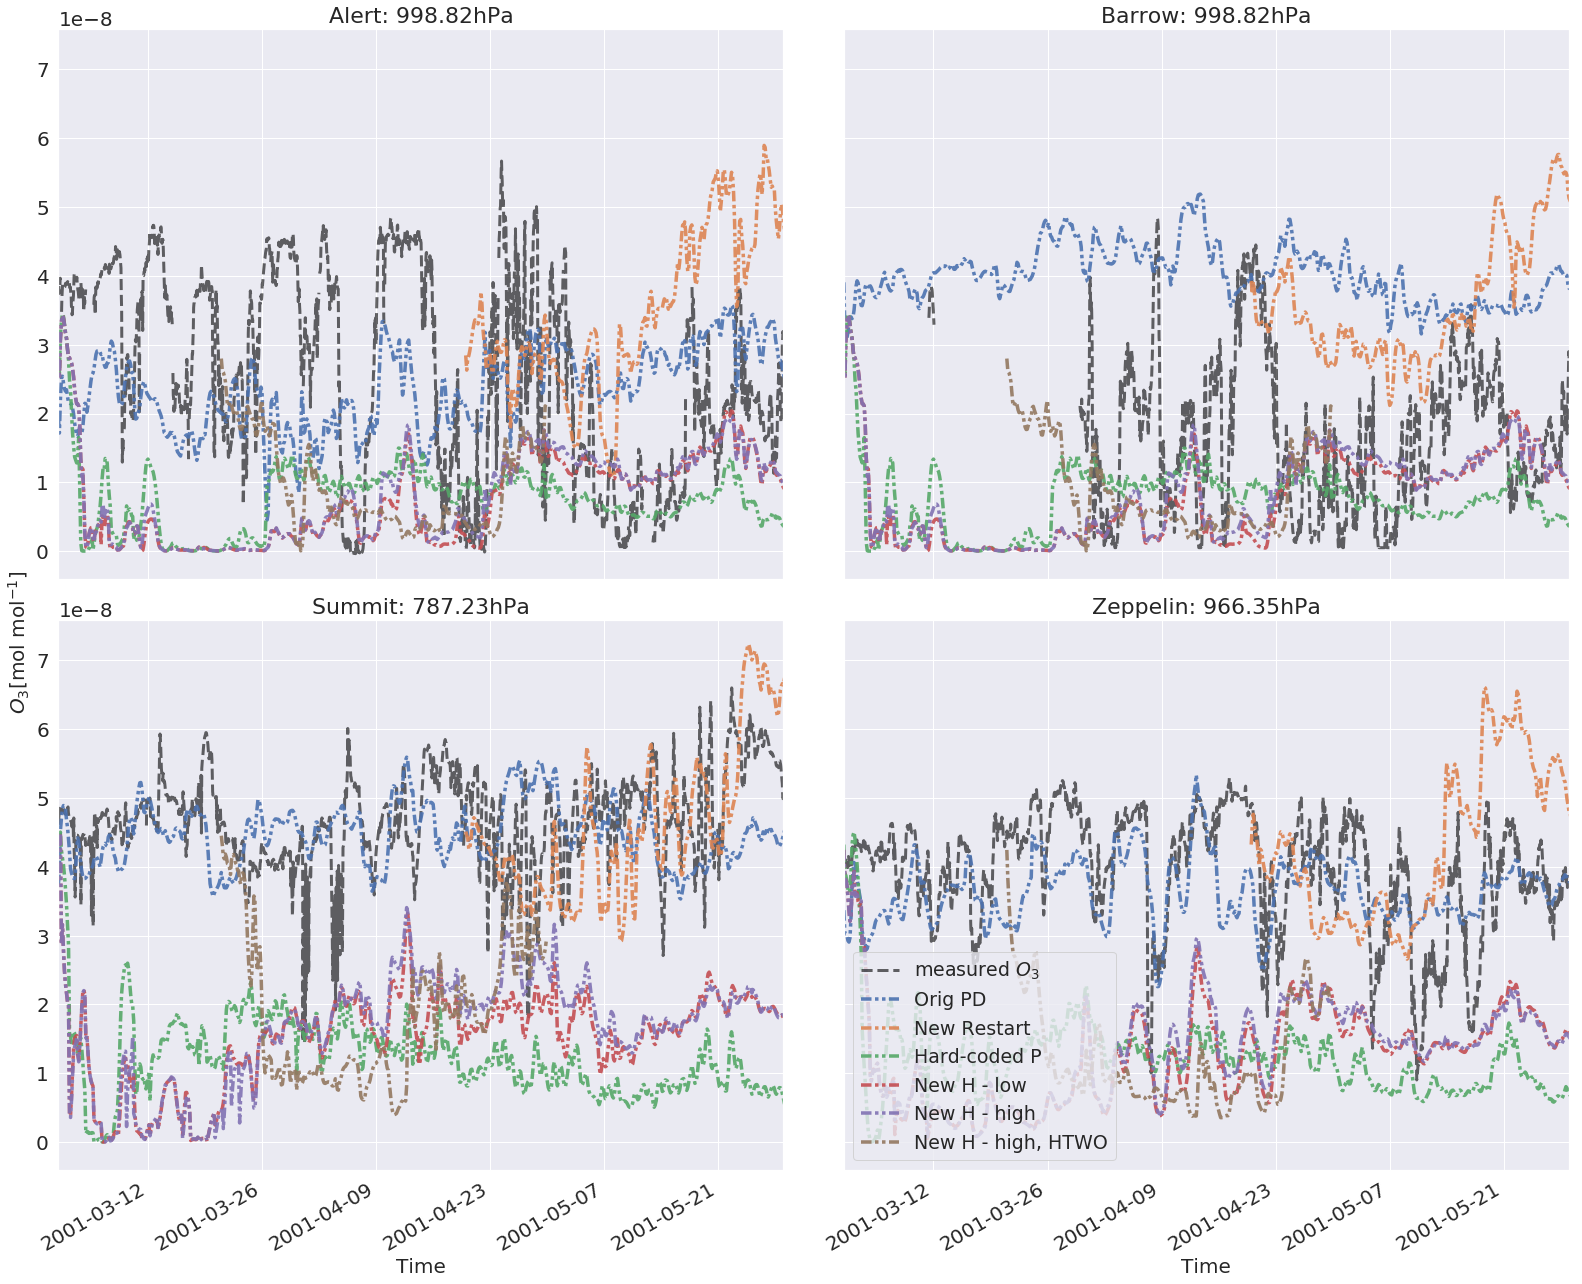
\includegraphics[width=\linewidth]{Chapter6_Results/images/ozone_2001_step3.png}
    \caption{Ozone measurements (black line) and model results from the original CTM3 (blue line) (these two are the same as in Figure \ref{fig:test_RemoveHetReacts}), test with new restart file from Section \ref{sec:step2_result} (orange line), hard-coded photodissociation rates (green line), new (low) Henry's law constant of $7.2\times10^{-1} M atm ^{-1}$ and $6100 K$ (pink line), new (high) Henry's law constant of $2.5\times10^{1} M atm ^{-1}$ and $370 K$ (purple line) and the latter ran at HTWO resolution (brown line) at the four different stations, Alert (top left), Barrow (top right), Summit (lower left) and Zeppelin (lower right) with available measurements in 2001. Model results are taken from the first model level at $998.82 hPa$. PD = present day, P = photolysis rate, H = Henry's Law}
    \label{fig:ozone_2001_step3}
\end{figure}